\documentclass[12pt,a4paper,oneside]{book}
\usepackage[a4paper, top=3cm, bottom=3cm]{geometry}
\usepackage[latin1]{inputenc}
\usepackage[brazil]{babel}
\usepackage{setspace}
\usepackage{fancyhdr}
\usepackage{tocloft}
\usepackage{multicol}
\usepackage{graphicx}


\begin{document}

% Capa
%-------------------------------------------------------------------------------
\pagestyle{empty}
\title{Guia de Estudos para Matem\'atica Discreta Mais}
\author{Eric Ara\'ujo \and Neumar Malheiros}
\maketitle


% General definitions for all Chapters
%-------------------------------------------------------------------------------
% Define Page style for all chapters
\pagestyle{fancy}
% Delete the current section for header and footer
\fancyhf{}
% Set custom header
\lhead[]{\thepage}
\rhead[\thepage]{}
% Set arabic (1,2,3...) page numbering
\pagenumbering{arabic}
% Set double spacing for the text
%\doublespacing


% Not enumerated chapter
%-------------------------------------------------------------------------------
\chapter*{Pref\'acio}

Este \'e o seu guia para cursar a disciplina Matem\'atica Discreta. Este guia est\'a organizado da seguinte forma.

%-------------------------------------------------------------------------------
\chapter*{Agradecimentos}

Este \'e o seu guia para cursar a disciplina Matem\'atica Discreta. Este guia est\'a organizado da seguinte forma.

% ToC
%-------------------------------------------------------------------------------
\newpage
% Include dots between chapter name and page number
\renewcommand{\cftchapdotsep}{\cftdotsep}
%Finally, include the ToC
\tableofcontents

% 
%-------------------------------------------------------------------------------

%----------------------------------------------------------
\addcontentsline{toc}{chapter}{Ementa}
\chapter*{Ementa}

Os t\'opicos estudados neste curso est\~ao divididos em seis partes.

neumar

\begin{enumerate}
\item L\'ogica e Demonstra\c{c}\~oes
\begin{enumerate}
\item L\'ogica Proposicional
\item Predicados e quantificadores
\item M\'etodos (t\'ecnicas) de demonstra\c{c}\~ao
\end{enumerate}

\item Teoria dos N\'umeros
\begin{enumerate}
\item Sequ\^encias e somat\'orios (conjuntos enumer\'aveis)
\item Os n\'umeros inteiros e a divis\~ao
\item Os n\'umeros primos e os M\'aximos divisores comuns
\end{enumerate}

\item Indu\c{c}\~ao e Recursividade
\begin{enumerate}
\item Indu\c{c}\~ao Matem\'atica
\item Indu\c{c}\~ao completa e boa ordena\c{c}\~ao
\item Defini\c{c}\~oes recursivas e indu\c{c}\~ao estrutural
\item Rela\c{c}\~oes de recorr\^encia
\end{enumerate}

\item Contagem
\begin{enumerate}
\item Conceitos b\'asicos de contagem
\item Princ\'ipio da casa dos pombos
\item Permuta\c{c}\~oes e combina\c{c}\~oes
\item Princ\'ipio da inclus\~ao-exclus\~ao
\end{enumerate}

\item Rela\c{c}\~oes
\begin{enumerate}
\item Fun\c{c}\~oes
\item Rela\c{c}\~oes e suas propriedades
\item Fecho de rela\c{c}\~oes
\item Rela\c{c}\~oes de equival\^encia
\item Ordens parciais
\end{enumerate}

\item Grafos
\begin{enumerate}
\item Conceitos b\'asicos em Grafos
\item Representa\c{c}\~ao e Isomorfismo
\item Concectividade
\item Caminhos eulerianos e hamiltonianos
\item \'Arvores
\end{enumerate}
\end{enumerate}

\addcontentsline{toc}{chapter}{Avalia\c{c}\~ao}
\chapter*{Avalia\c{c}\~ao Mudada}

Teremos 3 tipos de atividades avaliativas:

\begin{itemize}
\item \textbf{Prova}: Avalia\c{c}\~ao individual, escrita e sem consulta.
\item \textbf{Desafio}: Avali\c{c}\~ao em grupo, escrita e com consulta.
\item \textbf{Projeto de Programa}: Trabalho pr\'atico de programa\c{c}\~ao em grupo.
\end{itemize}

Os pesos de cada atividade avaliativa est\~ao definidos na Tabela \ref{tab:avaliacao}

\begin{table}[htdp]
\caption{Atividades Avaliativas}
\begin{center}
\begin{tabular}{lr}
\hline
\textbf{Atividade} & \textbf{Peso} \\
\hline
Prova 1 & 30\% \\
\hline
Prova 2 & 30\% \\
\hline
Desafios & 30\% \\
\hline
Projetos de Programa\c{c}\~ao & 10\% \\
\hline
\end{tabular}
\end{center}
\label{tab:avaliacao}
\end{table}%

A nota final ($NF$) no curso ser\'a calculada com a seguir:
\begin{equation}
NF = NP1 * 0,3 +  NP2 * 0,3 +  MD * 0,3 + MP * 0,1,
\end{equation}

onde $NP1$ \'e a nota na Prova 1, $NP2$ \'e a nota na Prova 2, $MD$ \'e a m\'edia aritm\'etica das notas nos desafios e $MP$ \'e a m\'edia aritm\'etica das notas nos projetos de programa\c{c}\~ao.

Para ser aprovado, o estudante precisa obter $NF \geq 60$.


\addcontentsline{toc}{chapter}{Plano do Curso}
\chapter*{Plano do Curso}


\begin{table}[htdp]
\caption{Plano do Curso}
\begin{center}
\begin{tabular}{cl}
\hline
\textbf{Aula} & \textbf{Atividade} \\
\hline
1 & Apresenta\c{c}\~ao do curso e L\'ogica Proposicional \\
\hline
2 & Predicados e quantificadores \\
\hline
3 & M\'etodos (t\'ecnicas) de demonstra\c{c}\~ao \\
\hline
4 & Simulado para o Desafio \\
\hline
5 & \textbf{Atividade Avaliativa: Desafio 1} \\
\hline
6 & Sequencias e somatorios. \\
\hline
7 & Os n\'umeros inteiros e a divis\~ao\\
\hline
8 & Os n\'umeros primos e os M\'aximos divisores comuns \\
\hline
9 & Simulado para o Desafio \\
\hline
10 & \textbf{Atividade Avaliativa: Desafio 2}\\
\hline
11 & Indu\c{c}\~ao Matem\'atica e  Indu\c{c}\~ao completa e boa ordena\c{c}\~ao \\
\hline
12 & Defini\c{c}\~oes recursivas e indu\c{c}\~ao estrutural e Rela\c{c}\~oes de recorr\^encia\\
\hline
13 & Simulado para o Desafio \\
\hline
14 & \textbf{Atividade Avaliativa: Desafio 3} \\
\hline
15 & \textbf{Atividade Avaliativa: Prova 1} \\
\hline
16 &  Conceitos b\'asicos de contagem\\
\hline
17 & Permuta\c{c}\~oes e combina\c{c}\~oes \\
\hline
18 & Princ\'ipio da casa dos pombos e Princ\'ipio da inclus\~ao-exclus\~ao \\
\hline
19 & Simulado para o Desafio \\
\hline
20 & \textbf{Atividade Avaliativa: Desafio 4} \\
\hline
21 & Rela\c{c}\~oes e suas propriedades \\
\hline
22 & Fun\c{c}\~oes e Rela\c{c}\~oes de equival\^encia \\
\hline
23 & Fecho de rela\c{c}\~oes e Ordens parciais \\
\hline
24 & Simulado para o Desafio \\
\hline
25 & \textbf{Atividade Avaliativa: Desafio 5} \\
\hline
26 & Conceitos b\'asicos em Grafos \\
\hline
27 & Representa\c{c}\~ao e Isomorfismo \\
\hline
28 & Concectividade \\
\hline
29 & Caminhos eulerianos e hamiltonianos \\
\hline
30 &  \'Arvores \\
\hline
31 & \'Arvores \\
\hline
32 & Simulado para o Desafio \\
\hline
33 & \textbf{Atividade Avaliativa: Desafio 6} \\
\hline
34 & \textbf{Atividade Avaliativa: Prova 2} \\
\hline

%\item 
%\item 
%\item %\item 
%\item �?rvores

\end{tabular}
\end{center}
\label{default}
\end{table}%







%----------------------------------------------------------
% If the chapter ends in an odd page, you may want to skip having the page
%  number in the empty page
%\newpage
%\thispagestyle{empty}


% Capitulos para cada aula
% First enumerated chapter
%-------------------------------------------------------------------------------

%!TEX root =  ../guia-MD.tex

\chapter{Assunto}

\section*{Prepare-se!}

Nesta aula, estudaremos os conceitos b�sicos sobre assunto.

Antes desta aula, o estudante deve ler o livro texto da disciplina \cite{rosen09}.

\section*{Notas de Aula}

\begin{minipage}{0.7\linewidth}

Inserir  notas de aula. Inserir  notas de aula. Inserir  notas de aula. Inserir  notas de aula. Inserir  notas de aula. Inserir  notas de aula. Inserir  notas de aula. Inserir  notas de aula. Inserir  notas de aula. Inserir  notas de aula. Inserir  notas de aula. Inserir  notas de aula. 

Inserir  notas de aula. Inserir  notas de aula. Inserir  notas de aula. Inserir  notas de aula. Inserir  notas de aula. Inserir  notas de aula. Inserir  notas de aula. Inserir  notas de aula. Inserir  notas de aula. Inserir  notas de aula. Inserir  notas de aula. Inserir  notas de aula. Inserir  notas de aula. Inserir  notas de aula. Inserir  notas de aula. Inserir  notas de aula. Inserir  notas de aula. Inserir  notas de aula. Inserir  notas de aula. Inserir  notas de aula. Inserir  notas de aula. Inserir  notas de aula. Inserir  notas de aula. Inserir  notas de aula. Inserir  notas de aula. Inserir  notas de aula. Inserir  notas de aula. Inserir  notas de aula. Inserir  notas de aula. Inserir  notas de aula. Inserir  notas de aula. Inserir  notas de aula. Inserir  notas de aula. Inserir  notas de aula. Inserir  notas de aula.

Como na Figura \ref{fig:type}

Inserir  notas de aula. Inserir  notas de aula. Inserir  notas de aula. Inserir  notas de aula. Inserir  notas de aula. Inserir  notas de aula. Inserir  notas de aula. Inserir  notas de aula. Inserir  notas de aula. Inserir  notas de aula. Inserir  notas de aula. Inserir  notas de aula. Inserir  notas de aula. Inserir  notas de aula. Inserir  notas de aula. Inserir  notas de aula. Inserir  notas de aula. Inserir  notas de aula. Inserir  notas de aula. Inserir  notas de aula. Inserir  notas de aula. 

Teste acentos. Computa��o. L�gica.

\end{minipage}

\begin{figure}[htbp]
\begin{center}
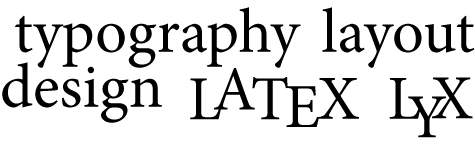
\includegraphics[scale=0.4]{aulas/figuras/type.png}
\caption{Teste.}
\label{fig:type}
\end{center}
\end{figure}


\newpage
\section*{Exerc�cios de Fixa��o}

\begin{enumerate}
\item $P = NP$ ?
\item Qual a l�gica do universo e todas as coisas al�m?
\end{enumerate}

%%!TEX root =  ../guia-MD.tex

\chapter{L�gica Proposicional}

\section*{Prepare-se!}

Nesta aula, estudaremos os conceitos b�sicos sobre assunto.

Antes desta aula, o estudante deve ler o livro texto da disciplina \cite{rosen09}.

\section*{Notas de Aula}

\begin{minipage}{0.7\linewidth}

Inserir  notas de aula. Inserir  notas de aula. Inserir  notas de aula. Inserir  notas de aula. Inserir  notas de aula. Inserir  notas de aula. Inserir  notas de aula. Inserir  notas de aula. Inserir  notas de aula. Inserir  notas de aula. Inserir  notas de aula. Inserir  notas de aula. 

Inserir  notas de aula. Inserir  notas de aula. Inserir  notas de aula. Inserir  notas de aula. Inserir  notas de aula. Inserir  notas de aula. Inserir  notas de aula. Inserir  notas de aula. Inserir  notas de aula. Inserir  notas de aula. Inserir  notas de aula. Inserir  notas de aula. Inserir  notas de aula. Inserir  notas de aula. Inserir  notas de aula. Inserir  notas de aula. Inserir  notas de aula. Inserir  notas de aula. Inserir  notas de aula. Inserir  notas de aula. Inserir  notas de aula. Inserir  notas de aula. Inserir  notas de aula. Inserir  notas de aula. Inserir  notas de aula. Inserir  notas de aula. Inserir  notas de aula. Inserir  notas de aula. Inserir  notas de aula. Inserir  notas de aula. Inserir  notas de aula. Inserir  notas de aula. Inserir  notas de aula. Inserir  notas de aula. Inserir  notas de aula.

Como na Figura \ref{fig:type}

Inserir  notas de aula. Inserir  notas de aula. Inserir  notas de aula. Inserir  notas de aula. Inserir  notas de aula. Inserir  notas de aula. Inserir  notas de aula. Inserir  notas de aula. Inserir  notas de aula. Inserir  notas de aula. Inserir  notas de aula. Inserir  notas de aula. Inserir  notas de aula. Inserir  notas de aula. Inserir  notas de aula. Inserir  notas de aula. Inserir  notas de aula. Inserir  notas de aula. Inserir  notas de aula. Inserir  notas de aula. Inserir  notas de aula. 

Teste acentos. Computa��o. L�gica.

\end{minipage}

\begin{figure}[htbp]
\begin{center}
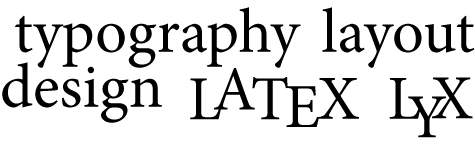
\includegraphics[scale=0.4]{aulas/figuras/type.png}
\caption{Teste.}
\label{fig:type}
\end{center}
\end{figure}


\newpage
\section*{Exerc�cios de Fixa��o}

\begin{enumerate}
\item $P = NP$ ?
\item Qual a l�gica do universo e todas as coisas al�m?
\end{enumerate}


%%%% Referencias
\bibliographystyle{plain}
\bibliography{referencias}

\end{document}